%!TEX root = ../article.tex
% \section{Introduction}
Nowadays, the widely used location-acquisition devices lead to an explosive increase of the movement data which is recorded in the form of trajectories. 
\NH{For example, the taxis trajectory is one of the common studied movement data which is always considered as the representative of human movement trace in a city. Using the taxi dataset in Shenzhen as an example, more than **(size) of trajectory data can be collected every day, which records (distance) by sampling locations.}
The analysis over these databases can be applied in many fields such as traffic management~\cite{wang2014visual}, urban planning, route recommendation~\cite{zheng2011learning} and location-based services~\cite{liu2016smartadp, zheng2010collaborative}. 

Visualizing trajectories is a challenging task. The most popular and conventional method is the line-based visualization~\cite{chen2015survey}: connecting the passing points of movement objects by polylines. The current visualization tools always don't scale well for the presentation of very large trajectory dataset due to the two challenges, visual clutter and limited rendering speed, which hinders the abilities of human-users for interactively exploring the dataset and identifying the movement patterns. 
In recent years, most of the visualization research works mainly try to address the visual clutter issue by proposing new techniques such as the spatial aggregation~\cite{zeng2013visualizing, von2015mobilitygraphs}, edge bundling~\cite{zeng2019route, thony2015vector} and density map~\cite{lampe2011interactive, scheepens2011interactive}. Instead, in this paper, we focus on the challenge of inefficient rendering in the large trajectory dataset by involving data sampling techniques. 


\NH{Using ** dataset as an example, figure~\ref{fig:rendering_time} demonstrates the rendering time at each dataset size, which shows that normal method takes more than ** minutes to generate the visualization, which is far beyond the human-acceptable response time for the interactive exploration~\cite{shneiderman1984response}.}

\begin{figure}[t]
	\centering
	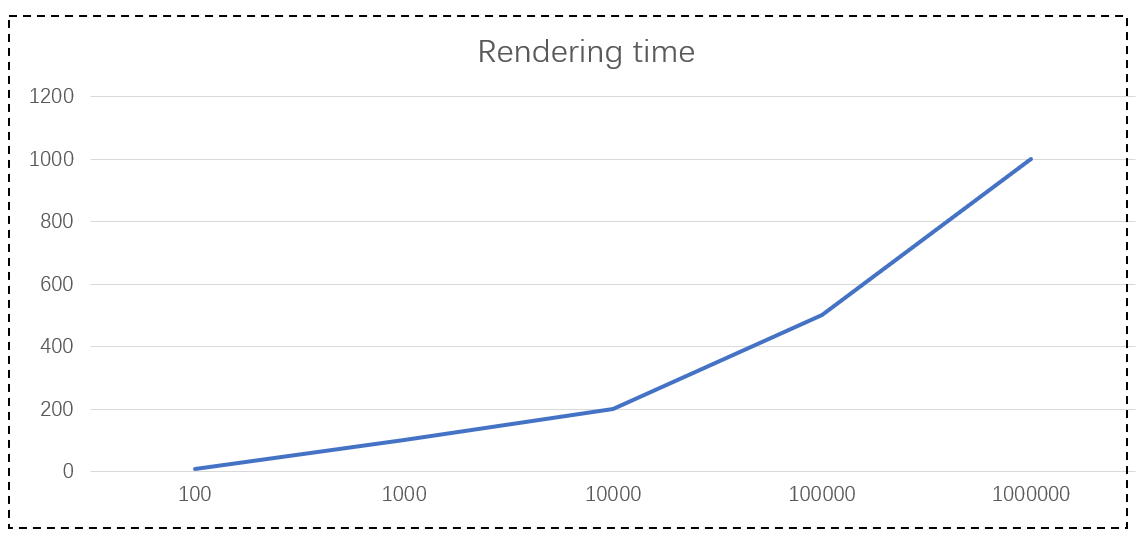
\includegraphics[width=0.49\textwidth]{pictures/introduction/rendering.png}
	\vspace{-5mm}
	\caption{\NH{x-data size; y-rendering time} }
	\vspace{-5mm}
	\label{fig:rendering_time}
\end{figure}

To handle the big dataset, many visualization products such as Spotfire~\cite{} and Tableau~\cite{} support advanced database management systems as a ``backend'' for the efficient data processing the query.
One work closely related to ours is ScalaR~\cite{battle2013dynamic}, which adds a reduction layer between visualization layer and data management layer. The reduction layer uses an uniform random sampling method to sample data once the query results are large enough, thus to reduce the amount of data to be visualized.
Further more, Park et al. propose VAS~\cite{park2016visualization} which implements new sampling techniques to guarantee the visual quality. However, these sampling techniques are designed for the simple dataset, and have been approved effective in scatter plot or map plot. However, the trajectory sampling is more challenge due to the complexity of data form(e.g. varying lengths, lack of compact representation, difficulty in measuring the similarity) that makes traditional density-biased sampling techniques inappropriate.

In our method, we extend the motivation of visualization-aware sampling to trajectory dataset. We propose a novel sampling strategy, \textbf{v}isualization \textbf{a}ware \textbf{t}rajectory \textbf{s}ampling(VATS), that produces high-visual-quality line-based trajectory visualization at certain degree(\QM{arbitrary}) zooming resolutions. 
\QM{In this paper, we first proposed the visual fidelity loss function which effectively evaluates the visual loss of the sampling method. Then we minimize the loss function by transforming this problem to an optimization problem. Several solutions for efficiently solving the optimization problem are discussed.}
Figure~\ref{fig:compare} depicts an comparison among the ground truth,  uniform random sampling and our proposed method. By limiting the sampling set size, the proposed method generates a higher-fidelity visualization and support the multi-resolution very well.   

\begin{figure}[t]
	\centering
	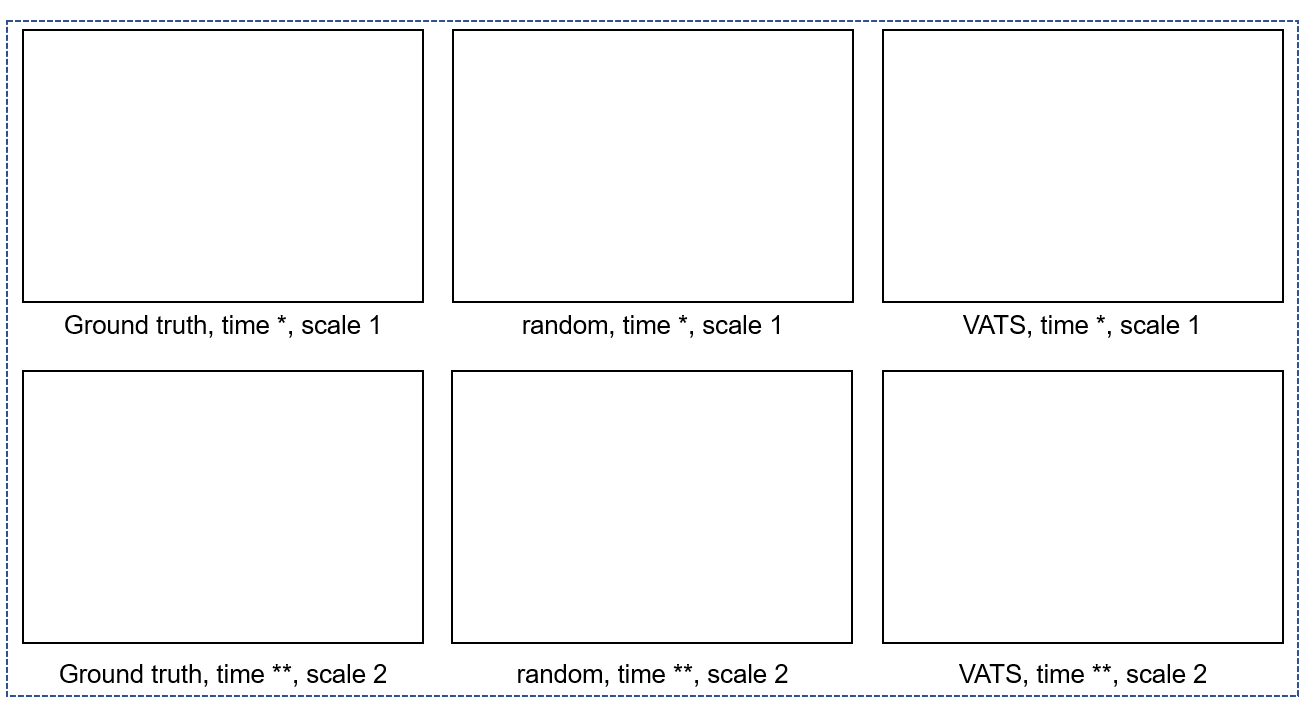
\includegraphics[width=0.49\textwidth]{pictures/introduction/compare.png}
	\vspace{-5mm}
	\caption{\NH{three columns (ground truth, random sampling, proposed method), two rows(top level, middle level)} }
	\vspace{-5mm}
	\label{fig:compare}
\end{figure}

We summarize our contribution as follows:
\setlist{nolistsep}
\begin{itemize}[noitemsep]
  \item We formulate VATS as an optimization problem.
  \item We prove VAST problem is NP-hard and offer an efficient approximation algorithms. 
  \item We conduct several experiments using real-world data to demonstrate the effectiveness of the proposed method in comparison with random uniform sampling.
\end{itemize}


The remaining parts are constructed as follows: section 2 discusses the related work. In section 3, we identify the specific problem and provide an overview of our solution. We define the problem and propose the solution in the section 4 and 5. The implementation and experiment setting are introduced in section 6. 
In section 7, we conduct case studies and user studies to evaluate our approach. Finally, we conclude this paper and propose the possible future directions in section 8.
